\chapter{Detailed Analysis of Subcellular Localisation of Human and Bovine IFIT Proteins in the Context of RSV Inclusion Bodies}

\section{Introduction and Aims}
Add intro about what we think it’s happening with IBs and pIBs \newline
Using pIBs as simpler model (only N+P+ cellular components) -> h/bRSV infections -> overexpression during infection

\begin{figure}
    \centering
    \includegraphics[width=1\linewidth]{08. Chapter 3//Figs//01. Introduction/IB-zooms.pdf}
    \caption[Representative Infection Zoom.]{\textbf{Representative Infection Zoom.} asdf asdf asdf asdf asdf asdf sdfgsdfg}
    \label{Representative Infection Zoom}
\end{figure}

\section{Results}
\subsection{IFIT1} \label{IFIT1}
\subsubsection{Nascent Human and Monkey IFIT1 in a Simplified System of pseudo-IBs} \label{Nascent Human and Monkey IFIT1 in a Simplified System of pseudo-IBs}
\myparagraph{293t hnhp}

\begin{figure}
    \centering
    \includegraphics[width=1\linewidth]{08. Chapter 3//Figs//02. IFIT1/01. endo_human.pdf}
    \caption[i1 293t hnhp]{i1 293t hnhp}
    \label{i1 293t hnhp}
\end{figure}

Detecting magenta: endogenous human IFIT1 \newline
Detecting cyan: human pIB \newline
Cell Line: 293T \newline
Treatment: hNhP \newline

Nascent human IFIT1 seems to be diffused through the pIB structure i.e., the signal intensity and distribution between cytoplasmic and pIB staining is identical.  

\myparagraph{vero hnhp}
Detecting magenta: endogenous monkey IFIT1 \newline
Detecting cyan: human pIB \newline
Cell Line: VERO \newline
Treatment: hNhP \newline

Endogenous monkey IFIT1 displays colocalization with human pIB structures (top panel), or inclusion within the structures (bottom panel). Monkey IFIT1 signal is also excluded from the pIB filamentous network (top panel; shown by arrows). This suggests that the colocalization is not caused by mere interaction with N or P but its dependant on the integrity of pIBs. These data are supported by z stack measurements.  

\begin{figure}
    \centering
    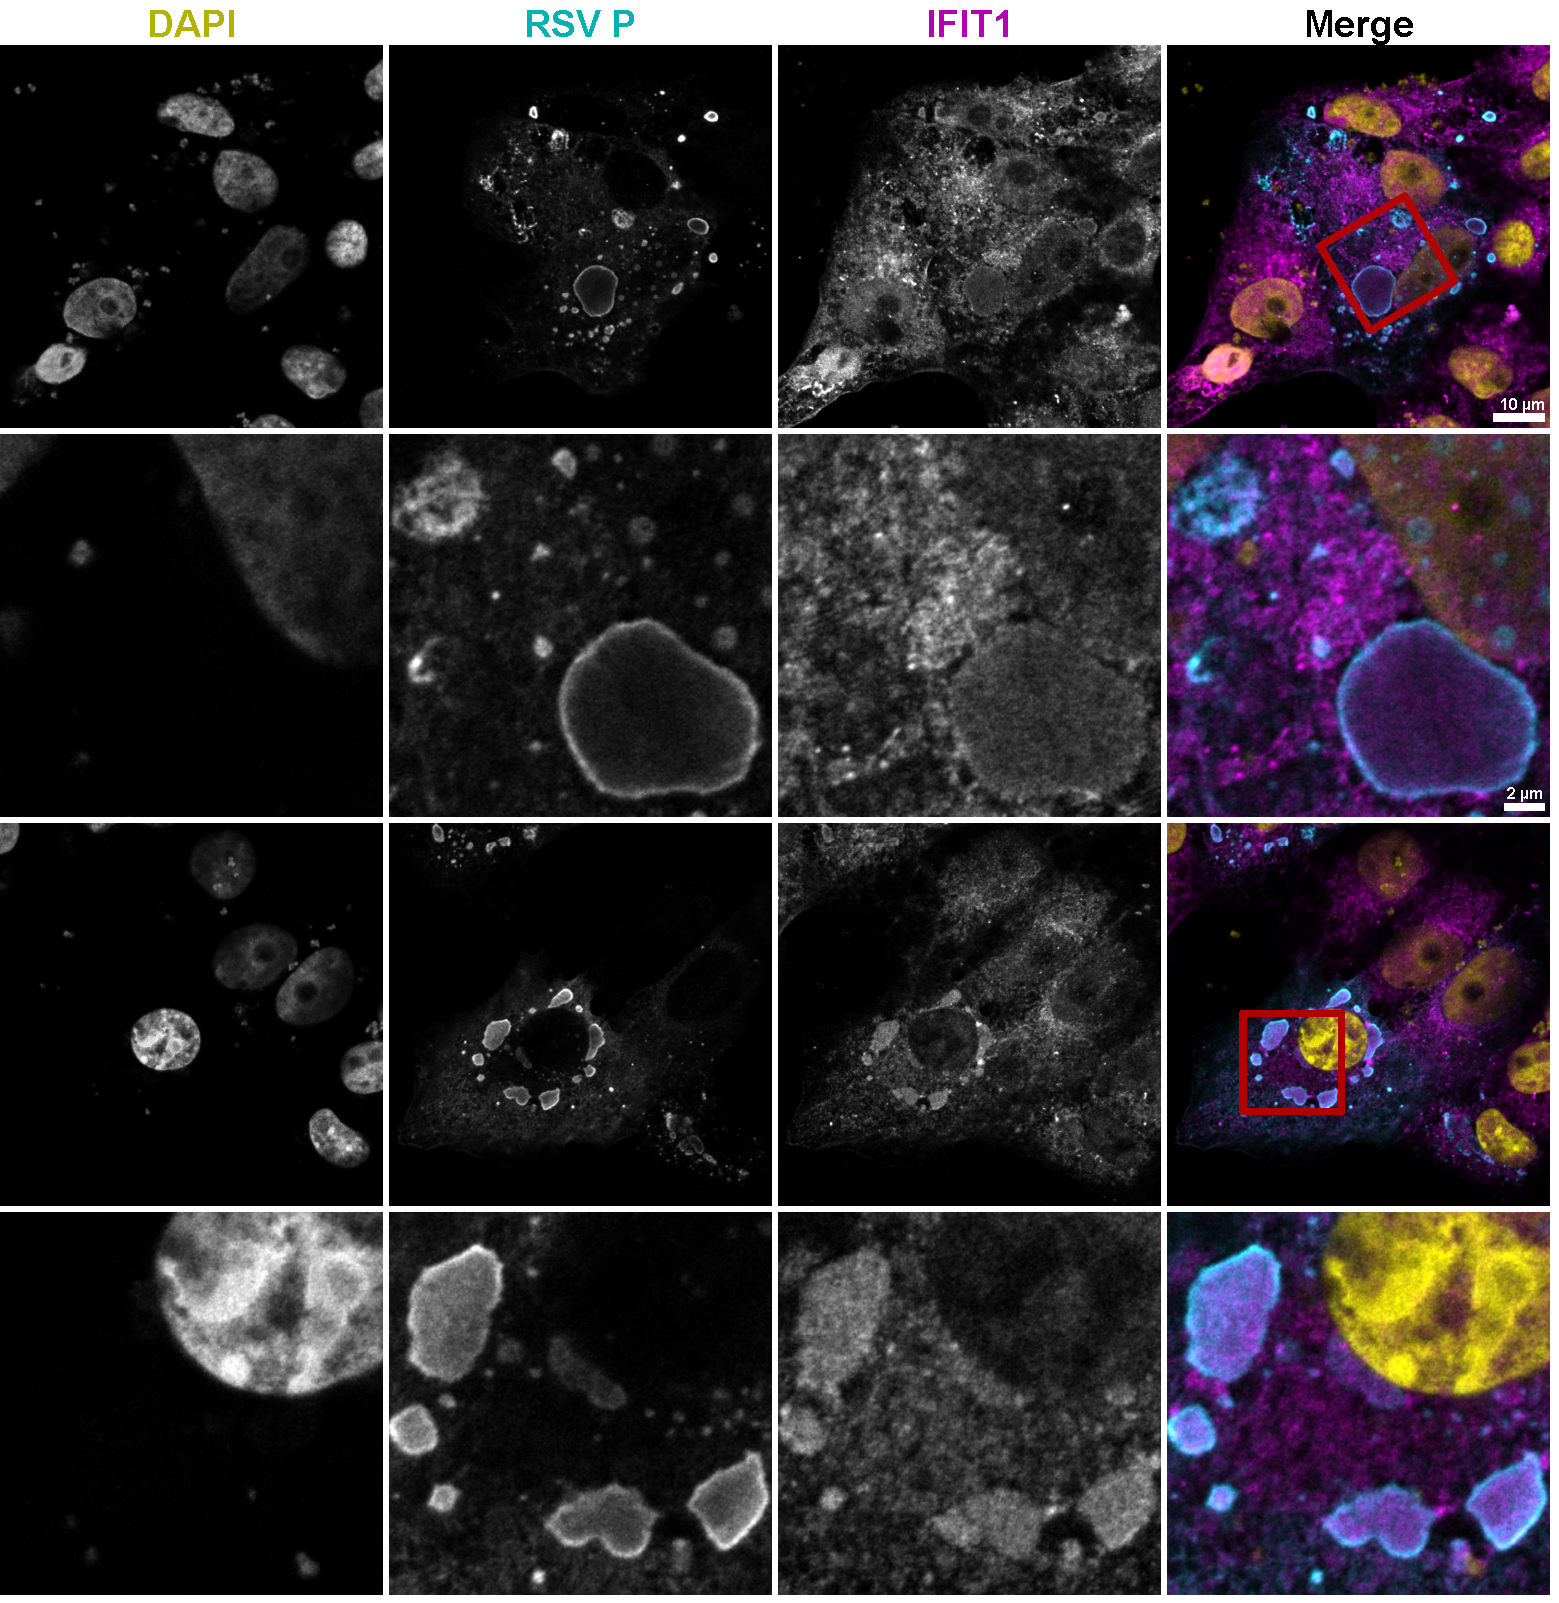
\includegraphics[width=1\linewidth]{08. Chapter 3/Figs/02. IFIT1/02. endo_monkey.pdf}
    \caption[i1 vero hnhp]{i1 vero hnhp}
    \label{i1 vero hnhp}
\end{figure}


\myparagraph{vero bnbp}
Cell Line: VERO \newline
Treatment: bNbP \newline
Detecting magenta: endogenous monkey IFIT1 \newline
Detecting cyan: bovine pIB \newline

In the context of bovine pIB structures, nascent monkey IFIT1 seems to colocalise with the edges of the structures (highlighted by the arrows). Consistent to human pIB data, nascent monkey IFIT1 is excluded from filamentous pIB network.


\begin{figure}
    \centering
    \includegraphics[width=1\linewidth]{08. Chapter 3/Figs/02. IFIT1/03. endo_monkey_bovine-pIB.pdf}
    \caption[i1 vero bnbp]{i1 vero bnbp}
    \label{i1 vero bnbp}
\end{figure}

\subsubsection{Nascent Human and Bovine IFIT1 Localisation During h/bRSV Infection} \label{Nascent Human and Bovine IFIT1 Localisation During h/bRSV Infection}
\myparagraph{hIFIT1 Localisation During hRSV Infection} \label{hIFIT1 Localisation During hRSV Infection}
\mysubparagraph{a549 hrsv}
Detecting magenta: endogenous human IFIT1 \newline
Detecting cyan: human IB \newline
Cell Line: A549 \newline
Treatment: hRSV \newline

Nascent human IFIT1 shows several distinct phenotypes with respect to the hRSV IB interaction. IFIT1 is either concentrated inside the structure (top panel), concentrated on the edge of IB ring (2nd and 3rd panels)  , excluded from the IB structure (4th panel),  or is diffused evenly between the cytoplasm and IB structure (bottom panel).

\begin{figure}
    \centering
    \includegraphics[width=1\linewidth]{08. Chapter 3/Figs/02. IFIT1/04. human infection.png}
    \caption[i1 a549 hrsv]{i1 a549 hrsv}
    \label{i1 a549 hrsv}
\end{figure}

\mysubparagraph{a549 brsv}
some text

\begin{figure}
    \centering
    \includegraphics[width=0.5\linewidth]{06. Chapter 1//Figs/00. placeholder.png}
    \caption[i1 a549 brsv]{i1 a549 brsv}
    \label{i1 a549 brsv}
\end{figure}

\mysubparagraph{beas2b hrsv}
Detecting magenta: endogenous human IFIT1 \newline
Detecting cyan: human IB \newline
Cell Line: BEAS2B \newline
Treatment: hRSV \newline

\begin{figure}
    \centering
    \includegraphics[width=1\linewidth]{08. Chapter 3/Figs/02. IFIT1/05. beas2b hrsv.png}
    \caption[i1 beas2b hrsv]{i1 beas2b hrsv}
    \label{i1 beas2b hrsv}
\end{figure}

\myparagraph{bIFIT1 Localisation During h/bRSV Infection} \label{bIFIT1 Localisation During h/bRSV Infection}
\mysubparagraph{mdbk hrsv}
some text

\begin{figure}
    \centering
    \includegraphics[width=0.5\linewidth]{06. Chapter 1//Figs/00. placeholder.png}
    \caption[i1 mdbk hrsv]{i1 mdbk hrsv}
    \label{i1 beas2b brsv}
\end{figure}

\mysubparagraph{mdbk brsv}
Detecting magenta: endogenous bovine IFIT1 \newline
Detecting cyan: bovine IB \newline
Cell Line: MDBK \newline
Treatment: bRSV dSH + bIFNa \newline

Nascent bovine IFIT1 in the context of bRSV infection has been observed to localise with the respect of IB in three distinct spaces. We observed it either concentrated inside the central point of the IB structure, while having reduced signal on the inner IB edge, compared to the cytoplasm (top and bottom panels), being excluded from the IB structure (3rd panel), or colocalising on the inner edge of the IB structure while having reduced signal in the middle of the structure compared to cytoplasm, or the edge staining (2nd panel).

\begin{figure}
    \centering
    \includegraphics[width=1\linewidth]{08. Chapter 3/Figs/02. IFIT1/06. mdbk brsv.png}
    \caption[i1 mdbk brsv]{i1 mdbk brsv}
    \label{i1 mdbk brsv}
\end{figure}

\mysubparagraph{bt brsv}
some text

\begin{figure}
    \centering
    \includegraphics[width=0.5\linewidth]{06. Chapter 1//Figs/00. placeholder.png}
    \caption[i1 bt brsv]{i1 bt brsv}
    \label{i1 bt brsv}
\end{figure}

\subsubsection{Exogenously Expressed hIFIT1-FLAG During RSV Infection} \label{Exogenously Expressed hIFIT1-FLAG During RSV Infection}
\myparagraph{hi1 + hrsv brsv}
Detecting magenta: exogenous human IFIT1-FLAG \newline
Detecting cyan: h/bIB \newline
Cell Line: VERO \newline
Treatment: h/bRSV-GFP \newline

Overexpressed hIFIT1-FLAG colocalises with both human and bovine RSV IBs. This data is supported by evidence from z stacks.

\begin{figure}
    \centering
    \includegraphics[width=1\linewidth]{08. Chapter 3/Figs/02. IFIT1/07. hi1 hrsv brsv.png}
    \caption[hi1 + hrsv brsv]{hi1 + hrsv brsv}
    \label{hi1 + hrsv brsv}
\end{figure}

\myparagraph{bi1 + hrsv brsv}
some text

\begin{figure}
    \centering
    \includegraphics[width=0.5\linewidth]{06. Chapter 1//Figs/00. placeholder.png}
    \caption[bi1 + hrsv brsv]{bi1 + hrsv brsv}
    \label{bi1 + hrsv brsv}
\end{figure}

\subsubsection{Summary} \label{Summary}
Endogenous human IFIT1 seems to be diffused through the human pIB structure. On the other hand, endogenous monkey IFIT1 forms an inclusion in human pIBs, colocalises with the edge of human and bovine pIBs and is excluded from the filamentous pIB network. This suggests that the colocalization is not caused by mere interaction with N or P but its dependant on the integrity of pIBs. In the context of infection, endogenous human IFIT1 concentrates within the human RSV IB structure; colocalises to the edge of the IB; is diffused through the structure and cytoplasm equally; or is excluded from the structure. This suggests that the interaction between human IFIT1 and hRSV IB is dynamic and depends on factors that we do not understand yet. In the case of endogenous bovine IFIT1 in the context of bRSV IBs, IFIT1 is either excluded from the structure; excluded from the IB inner edge but concentrated inside; or excluded from the centre of IB structure but concentrated on the inner edge of the structure. Overexpressed hIFIT1-FLAG in the context of h/bRSV infection colocalises to both human and bovine IB structures.
\subsection{IFIT3} \label{IFIT3}
\subsubsection{Nascent Human and Monkey IFIT3 in a Simplified System of pseudo-IBs} \label{Nascent Human and Monkey IFIT3 in a Simplified System of pseudo-IBs}
\myparagraph{vero hnhp}
Detecting magenta: endogenous monkey IFIT3 \newline
Detecting cyan: human pIB \newline
Cell Line: VERO \newline
Treatment: hNhP \newline

Nascent monkey IFIT3 seems to behave a if he pIB was not here. This means I has diffused phenotype. One exception is the top panel (shown with the arrow) which hints at concentrated IFIT3 at the edge of the pIBs. We do not know the localisation with respect to the pIB filaments as none were found in the slides. This data is as well supported by z stack measurements.

\begin{figure}
    \centering
    \includegraphics[width=1\linewidth]{08. Chapter 3/Figs/04. IFIT3/01. vero hnhp.png}
    \caption[i3 vero hnhp]{i3 vero hnhp}
    \label{i3 vero hnhp}
\end{figure}

\myparagraph{vero bnbp}
some text

\begin{figure}
    \centering
    \includegraphics[width=1\linewidth]{06. Chapter 1//Figs/00. placeholder.png}
    \caption[i3 vero bnbp]{i3 vero bnbp}
    \label{i3 vero bnbp}
\end{figure}

\subsubsection{Nascent Human and Bovine IFIT3 Localisation During h/bRSV Infection} \label{Nascent Human and Bovine IFIT3 Localisation During h/bRSV Infection}
\myparagraph{hIFIT3 Localisation During hRSV Infection} \label{hIFIT3 Localisation During hRSV Infection}
\mysubparagraph{a549 hrsv}
Detecting magenta: endogenous human IFIT3 \newline
Detecting cyan: human IB \newline
Cell Line: A549 \newline
Treatment: hRSV \newline

Nascent human IFIT3 seems to have mainly diffused phenotype (top and bottom panel) with occasional exclusion without any marked IFIT3 concentration adjacent to the IB structure (middle panel).

\begin{figure}
    \centering
    \includegraphics[width=1\linewidth]{08. Chapter 3/Figs/04. IFIT3/02. a549 hrsv.png}
    \caption[i3 a549 hrsv]{i3 a549 hrsv}
    \label{i3 a549 hrsv}
\end{figure}

\mysubparagraph{a549 brsv}
some text

\begin{figure}
    \centering
    \includegraphics[width=0.5\linewidth]{06. Chapter 1//Figs/00. placeholder.png}
    \caption[i3 a549 brsv]{i3 a549 brsv}
    \label{i3 a549 brsv}
\end{figure}

\mysubparagraph{beas2b hrsv}
Detecting magenta: endogenous human IFIT3 \newline
Detecting cyan: human IB \newline
Cell Line: BEAS2B \newline
Treatment: hRSV \newline

\begin{figure}
    \centering
    \includegraphics[width=1\linewidth]{08. Chapter 3/Figs/04. IFIT3/03. beas2b hrsv.png}
    \caption[i3 beas2b hrsv]{i3 beas2b hrsv}
    \label{i3 beas2b hrsv}
\end{figure}

\myparagraph{bIFIT3 Localisation During h/bRSV Infection} \label{bIFIT3 Localisation During h/bRSV Infection}
\mysubparagraph{mdbk hrsv}
some text

\begin{figure}
    \centering
    \includegraphics[width=0.5\linewidth]{06. Chapter 1//Figs/00. placeholder.png}
    \caption[i3 mdbk hrsv]{i3 mdbk hrsv}
    \label{i3 mdbk hrsv}
\end{figure}

\mysubparagraph{mdbk brsv}
Detecting magenta: endogenous bovine IFIT3 \newline
Detecting cyan: bovine IB \newline
Cell Line: MDBK \newline
Treatment: bRSV dSH + bIFNa \newline

In this experiment the nascent bovine IFIT3 was consistently concentrated inside IBs. In some IBs the IFIT3 signal showed signs of sub-concentrations within the inclusions (bottom panel; highlighted with arrows), resembling IBAGs (inclusion body associated granules).

Subsequent experiments did not recapitulate the IFIT3 inclusions. It however shows signal which is almost identical to what is observed with IFIT5 in MDBKs during bRSV infection i.e., decrease, but not complete abolishment of IFIT3 signal inside the IB structure (top panel), and IB boundary exclusion while maintaining similar levels of signal intensity between cytoplasmic and intra IB stain.

\begin{figure}
    \centering
    \includegraphics[width=1\linewidth]{08. Chapter 3/Figs/04. IFIT3/04. mdbk brsv.png}
    \caption[i3 mdbk brsv]{i3 mdbk brsv}
    \label{i3 mdbk brsv}
\end{figure}

\mysubparagraph{bt brsv}
some text

\begin{figure}
    \centering
    \includegraphics[width=0.5\linewidth]{06. Chapter 1//Figs/00. placeholder.png}
    \caption[i3 bt brsv]{i3 bt brsv}
    \label{i3 bt brsv}
\end{figure}

\subsubsection{Exogenously Expressed hIFIT3-FLAG During RSV Infection} \label{Exogenously Expressed hIFIT3-FLAG During RSV Infection}
\myparagraph{hi3 + hrsv brsv}
some text

\begin{figure}
    \centering
    \includegraphics[width=0.5\linewidth]{06. Chapter 1//Figs/00. placeholder.png}
    \caption[hi3 + hrsv brsv]{hi3 + hrsv brsv}
    \label{hi3 + hrsv brsv}
\end{figure}


\myparagraph{bi3 + hrsv brsv}
Cell Line: VERO \newline
Treatment: hRSV-GFP \newline
Detecting magenta: exogenous bovine IFIT3 \newline
Detecting cyan: human IB \newline

Overexpressed bIFIT3-FLAG was observed to colocalise with hRSV inclusion bodies (top panel; highlighted with arrows), as well as being excluded from the hRSV IBs, without any signs of IFIT3 signal on the periphery of the IB structures (middle and bottom panel). This data is supported by z stack measurements.

\begin{figure}
    \centering
    \includegraphics[width=1\linewidth]{08. Chapter 3/Figs/04. IFIT3/05. bi3 hrsv.png}
    \caption[bi3 + hrsv]{bi3 + hrsv}
    \label{bi3 + hrsv}
\end{figure}

Cell Line: VERO \newline
Treatment: bRSV-GFP \newline
Detecting magenta: exogenous bovine IFIT3 \newline
Detecting cyan: bovine IB \newline

Very similar phenotype is observed for overexpressed bIFIT3-FLAG in bRSV infected cells. We see colocalization with IB (top panel) as well as exclusion from the structure without any signs of IFIT3 signal on the periphery of the IB structure (bottom panel). This data is as well supported by z stack measurements.

\begin{figure}
    \centering
    \includegraphics[width=1\linewidth]{08. Chapter 3/Figs/04. IFIT3/06. bi3 brsv.png}
    \caption[bi3 + brsv]{bi3 + brsv}
    \label{bi3 + brsv}
\end{figure}

\subsubsection{Summary} \label{Summary}
Endogenous monkey IFIT3 seems to be diffuse through the human pIB structures (with maybe a small hint of colocalization). Nascent human IFIT3 during hRSV infection is either excluded from IB structure or is diffused through the structure. Occasionally it colocalises to the IB ring. Nascent bIFIT3 during bRSV infection either siphons inside IBs and shows sub-IB granules or is excluded from the IB boundary with slightly decreased signal inside of the IB. Overexpressed bIFIT3 behaves equally between hRSV and bRSV infection, that is it sometimes colocalises with the IB structure and sometimes is completely excluded from the structure.
\input{08. Chapter 3/Subchapters/03. IFIT5}

\subsection{Liquid-Liquid Phase Separation} \label{Liquid-Liquid Phase Separation}
Add stuff about the likelihood of IFIT and viral proteins and their propensity to phase separate \newline
This is using an online tool called PSPredictor


\section{Discussion}
pIBs and IBs are dynamic structures and that’s why we see variable interactions within the same IFIT experiments.